 
\documentclass[xcolor=svgnames]{beamer}
%
\usepackage[italian]{babel}

\usetheme{Singapore}
\setbeamertemplate{navigation symbols}{}
\setbeamertemplate{footline}[frame number]

%
\setbeamercolor{block body}{bg=AliceBlue}

\usepackage[all]{xy}
\usepackage{accents}
\usepackage{amsmath,amssymb}
\usepackage{array}
\usepackage{bibentry}
\usepackage{bm}
\usepackage{cancel}
\usepackage{comment}
\usepackage{etex}
\usepackage{macros}
\usepackage{mathscinet}
\usepackage{mathtools}
\usepackage{rotating}
\usepackage{tikz}

\hypersetup{
    colorlinks=true,
    linkcolor=blue,
    filecolor=magenta,      
    urlcolor=cyan
    }
\renewcommand{\newblock}{\relax} %% ??????????

%
%% Gianni macros
%

\DeclareMathOperator{\M}{\mathcal M}
\DeclareMathOperator{\eDeriv}{D_{\text{e}}}
\DeclareMathOperator{\grad}{grad}
\DeclareMathOperator{\mDeriv}{D_{\text{m}}}

\newcommand{\Bspaceat}[1]{B_{#1}}
\newcommand{\Bspace}[1]{B_{#1}}
\newcommand{\Ccs}[1]{C_0\left(#1\right)}
\newcommand{\Cexp}[1]{C_0^{(\cosh-1)}\left(#1\right)}
\newcommand{\Cinfcs}[1]{C_0^\infty\left(#1\right)}
\newcommand{\Cinfp}[1]{C_{\mathrm{p}}^\infty\left(#1\right)}
\newcommand{\Derivby}[1]{\frac{\Deriv}{d#1}}
\newcommand{\Lexp}[1]{L^{(\cosh-1)}\left(#1\right)}
\newcommand{\LlogL}[1]{L^{(\cosh-1)_*}\left(#1\right)}
\newcommand{\TMaxexp}{\operatorname{T}\Maxexp}
\newcommand{\WCexp}[1]{C_0^{1,(\cosh-1)}\left( #1 \right)}
\newcommand{\Wexp}[1]{W^{1,(\cosh-1)}\left(#1\right)}
\newcommand{\WlogL}[1]{W^{1,(\cosh-1)_*}\left(#1\right)}
\newcommand{\bgamma}{{\bm \gamma}}
\newcommand{\bnabla}{{\bm\nabla}}
\newcommand{\condexpectat}[3]{{\Expectation}_{#1}\left[#2 \middle| #3\right]}
\newcommand{\displacement}{\operatorname{\mathbb S}}
\newcommand{\eBspace}[1]{B_{#1}}
\newcommand{\eDerivby}[1]{\frac{\eDeriv}{d#1}}
\newcommand{\ehessianat}[2]{\prescript{e}{}\Hessian_{#1}{#2}}
\newcommand{\expbundle}{S\Maxexp}
\newcommand{\fullbundleat}[1]{\prescript{1}{}S^1\maxexpat{#1}}
\newcommand{\gaussdensity}{\gamma}
\newcommand{\gaussint}[2]{\int{#1} \gaussdensity(#2) \ d#2 \ }
\newcommand{\hullof}[1]{\operatorname{hull}\left(#1\right)}
\newcommand{\mDerivby}[1]{\frac{\mDeriv}{d#1}}
\newcommand{\maxmix}[1]{\prescript{*}{}{\Maxexp\left(#1\right)}}
\newcommand{\mhessianat}[2]{\prescript{m}{}\Hessian_{#1}{#2}}
\newcommand{\mixbundleat}[1]{\prescript{*}{}S\maxexpat{#1}}
\newcommand{\mixbundle}{\prescript{*}{}S\Maxexp}
\newcommand{\mixfiberat}[2]{{}^*S_{#1}\maxexpat{#2}}
\newcommand{\model}{\mathcal M}
\newcommand{\opensimplexon}[1]{\mathcal P_>\left(#1\right)}
\newcommand{\preBspaceat}[1]{\prescript{*}{}B_{#1}}
\newcommand{\preBspace}[1]{\prescript{*}{}B_{#1}}
\newcommand{\rosso}[1]{\textcolor{red}{#1}}
\newcommand{\sdomainat}[1]{\sdomain_{#1}}
\newcommand{\sdomain}{\mathcal S}
\newcommand{\simplexon}[1]{\mathcal P\left(#1\right)}
\newcommand{\tensorat}[3]{\prescript{#1}{}S^{#2}\maxexpat{#3}}

\renewcommand{\emph}{\rosso}
\renewcommand{\transport}[2]{{\mathbb U} _ {#1} ^ {#2}}

%
%% end Gianni's macros
%

\title{\it Intelligenza artificiale, apprendimento automatico, matematica, antropologia}

\author[G Pistone]{\bf Giovanni Pistone}

\institute[CCA]{
\includegraphics[height=4em]{pictures/deCastro-logo.pdf} \quad 
\includegraphics[height=4em]{pictures/logo Nuovo SEFIR con URL.png}}

\date{28 marzo 2023}

\begin{document} 
% 
\begin{frame}\frametitle{Un passo insieme onlus - Il salotto delle idee. Be curious.}  

\titlepage

\tiny 
web-page: \url{www.giannidiorestino.it} 

e-mail: \url{giovanni.pistone@carloalberto.org}

orcidID: 0000-0003-2841-788X

L'autore ringrazia De Castro Statistics e Nuovo SEFIR 

\nobibliography{tutto}%

\bibliographystyle{plain}

\end{frame}

\begin{frame}[plain]\tiny\frametitle{Sommario}
 Con intelligenza artificiale intendiamo oggi una collezione molto varia di tecnologie che vanno dal controllo automatico all’apprendimento automatico. In particolare l’apprendimento automatico ha avuto, molto recentemente, alcuni successi spettacolari che ora sono disponibili in applicazioni di uso di massa. Questi prodotti di successo si applicano al trattamento delle immagini, della lingua parlata, dei testi scritti. La caratteristica fondamentale di questi sistemi, che li distingue da quelli di controllo automatico, è che non sono completamente preprogrammati ma includono un sistema di apprendimento. Questo sistema di apprendimento si basa su almeno tre innovazioni metodologiche molto recenti. Queste sono le reti neurali, la sostituzione di regole sintattiche con regole semantiche, e l’uso sistematico di alte quantità di memoria. La gran parte della presentazione è dedicata ad illustrare queste tre metodologie. Concludo poi criticando le iperboli correnti secondo le quali saremmo di fronte ad una rivoluzione antropologica dovuta alla virtualizzazione. Sostengo, in linea con alcune analisi filosofiche, che siamo di fronte ad un ulteriore passo del caratteristico uso umano di dotarsi di un sistema di ritenzione della memoria sociale costituito sopratutto di utensili. Questi argomenti sono frutto dell’attività di ricerca svolta nell’ambito dell’associazione Nuovo SEFIR www.nuovo-sefir.it e della collaborazione con la filosofa Francesca dell’Orto.   
\end{frame}

\begin{frame}[plain]\tiny\frametitle{Bibliografia}
\begin{itemize}
 \item    F. Dell’Orto, G. Pistone. Big Data e metodo scientifico. in S. Rondinara (curatore) Si puo vivere senza scienza? SEFIR Citta Nuova 2022 (30-56).
     \item 
    G. Pistone. Dato e informazione. in M. Bernardoni (curatore) Cinque parole della scienza. Memoria e previsione, dato e informazione, tempo. EDB Nuovo SEFIR 2021 (133-150).
 \item   G. Pistone. Metodo in statistica. in S. Rondinara (curatore) Metodo. Nuovo SEFIR 2022 (16-20).
\end{itemize}

\end{frame}

\begin{frame}[plain]\tiny\frametitle{Biografia}
  Giovanni Pistone ha conseguito il dottorato in matematica nel 1975 (Rennes FR) e ha concluso la propria carriera accademica come professore di Probabilità del Politecnico di Torino nel 2010. Ora si occupa delle teorie geometriche e algebriche dell’informazione come affiliato della fondazione de Castro di Torino e come conferenziere. \`E socio dell’associazione Nuovo SEFIR. La sigla SEFIR significa Scienza e Fede sull’Interpretazione del Reale. La società è formata da intellettuali che discutono gli aspetti interdisciplinari delle loro rispettive specialità e presentano i propri risultati in pubblicazioni e convegni. Dal 2006 è predicatore locale ordinato della chiesa valdese (circuito di Torino).  
\end{frame}

\begin{frame}[plain]\small\frametitle{Intelligenza artificiale}

Specialmente sulla stampa, c'è oggi un gran parlare di intelligenza artificiale e delle sue conseguenze sull'economia e sulla nostra vita. 

Non sempre è ben chiaro quali sono le tecnologie che effettivamente presentano \emph{intelligenza} artificiale. 

Qui parlo della versione contemporanea (ultimi 10 anni) di questo concetto. Cioè, l'intelligenza artificiale di cui parliamo oggi non è quella di una volta. Non è la macchina in grado di battere un maestro a scacchi ma è piuttosto quella che è in grado di riconoscere le foto dei miei famigliari sul mio telefonino e mettere le mie foto in ordine.

Questa intelligenza artificiale moderna è essenzialmente legata ad un concetto di \emph{apprendimento automatico}. Questo apprendimento avviene per mezzo di metodi matematici di tipo statistico. La moderna intelligenza artificiale non si basa sulla teoria ma sulla pratica. 

Assimiglia più ad un professionista che \emph{valuta sulla base della propria esperienza} piuttosto che ad un esecutore preciso ed efficiente di regole esatte.

In questo senso sembra contraddire il normale paradigma scientifico basato sulla ricerca di leggi generali piuttosto che di esperienza accumulata. E inoltre mette a disaglio i professionisti che si sentono derubati delle loro specifiche capacità.

\end{frame}

\begin{frame}[plain,allowframebreaks]\small\frametitle{Generazione di testi: chat-GPT}

\begin{itemize}
\item OpenAI (=intelligenza artificiale aperta)  \url{https://openai.com/} è una ditta produttrice di software fondata del 2015 con lo scopo dichiarato di produrre friendly 
AI (=intelligenza artificiale amichevole)
    \item Il sistema \emph{chat-GPT} \url{https://chat.openai.com/chat} è disponibile previa registrazione in cui bisogna indicare indirizzo di posta elettronica, nome, numero di telefono.
    \item La suggestione è quella di una conversazione (chat). Non viene specificato quale è l'uso suggerito.
    \item \emph{GPT} significa 1) Generative 2) Pre-Trained. 
    \begin{enumerate}
        \item L'aggettivo ``generative'' indica un programma che produce nuovi casi simili ad una collezione di esempi. Per esempio, l'immagine di un gatto a partire da una raccolta di foto di gatti. O un testo a partire da una libreria di testi.
        \item L'aggettivo ``pre-trained'' significa che non è l'utente che deve addestrarlo, ma l'addestramento è già avvenuto in fabbrica.
    \end{enumerate} 
    \item Obbiettivo di questa presentazione è dare qualche informazione tecnica su questi due concetti: \emph{generazione} e \emph{addestramento}. Cioè discutere come funziona la moderna intelligenza artificiale dal punto di vista di uno, come me,  che si occupa degli algoritmi matematici che la fanno funzionare. Inoltre, vorrei argomentare che le problematiche culturali e politiche possono anch'esse essere discusse nel loro ambito proprio, che è quello filosofico.
    \item     Ecco un esempio di conversazione con Chat-GPT. Non mi è stato possibile prevedere di fare una dimostrazione dal vivo perché il sistema è spesso inaccessibile a causa dell'uso molto diffuso.
    \end{itemize}

    \newpage

    Si introducono delle domanda dalla tastiera e la macchina risponde sullo schermo.

    \vfill
    
    
\includegraphics[width=\textwidth]{pictures/Screenshot-chat-gpt.png}

\newpage

\begin{description}

\item[Giovanni] Buongiorno. Capisci l'italiano?

\item[chat-GPT] Sì, capisco l'italiano. Posso aiutarti con qualcosa?

\item[Giovanni] Conosci Un passo insieme ONLUS?

\item[chat-GPT] Sì, conosco Un Passo Insieme ONLUS. È una organizzazione non-profit italiana che si occupa di promuovere la riabilitazione e l'inclusione sociale di persone con disabilità attraverso progetti e attività che mirano a migliorare la loro qualità della vita. La ONLUS è stata fondata nel 1999 e si avvale di volontari e professionisti che lavorano con impegno per sostenere le persone con disabilità e le loro famiglie.

\item[Govanni] Cosa vuol dire disabilità?
Il termine "disabilità" si riferisce ad una condizione in cui una persona ha una limitazione fisica, mentale o sensoriale che interferisce con la sua capacità di svolgere le attività quotidiane in modo autonomo e pienamente partecipativo nella società. Ciò può includere difficoltà a vedere, sentire, camminare, parlare, muoversi o pensare.

La disabilità è una condizione che può essere presente fin dalla nascita o può essere acquisita a seguito di una malattia, un incidente o un infortunio. Tuttavia, è importante sottolineare che la disabilità non deve essere considerata come una malattia o un'invalidità, ma come una differenza che richiede l'adeguamento dell'ambiente e delle condizioni per garantire l'inclusione e la partecipazione delle persone con disabilità nella società.

\newpage

\item[Giovanni]
Dove leggi queste informazioni?

\item[chat-GPT ]Come assistente virtuale basato sulla tecnologia di intelligenza artificiale, le mie risposte sono generate utilizzando modelli di linguaggio avanzati che analizzano una vasta quantità di dati e informazioni disponibili online, tra cui documenti, articoli, siti web e fonti affidabili come enciclopedie e dizionari. Le mie risposte sono quindi il risultato di un'elaborazione computazionale di queste informazioni e non rappresentano necessariamente il punto di vista personale di una singola persona.

\newpage

\item[Giovanni]
L'omosessualità è una disabilità?

\tiny

\item[OpenAI] \emph{This content may violate our content policy. If you believe this to be in error, please submit your feedback — your input will aid our research in this area.}

\small

\item[chat-GPT]
No, l'omosessualità non è considerata una disabilità. Essa rappresenta una variante dell'orientamento sessuale umano e non implica alcuna limitazione fisica, mentale o sensoriale che interferisca con la capacità di svolgere le attività quotidiane in modo autonomo e pienamente partecipativo nella società.

La comunità medica e scientifica ha affermato che l'omosessualità non è una malattia o un disturbo mentale, bensì una normale espressione dell'orientamento sessuale umano. Infatti, l'Organizzazione Mondiale della Sanità (OMS) ha rimosso l'omosessualità dalla lista delle malattie mentali nel 1990, e molte organizzazioni a livello mondiale si sono espresse in modo chiaro sulla non patologicità dell'omosessualità.

\newpage

\item[Giovanni]
Serve pregare alle persone con disabilità?

\item[chat-GPT] La scelta di pregare o meno alle persone con disabilità dipende dalle loro credenze e desideri personali, così come dalle circostanze specifiche. Alcune persone con disabilità possono trovare conforto e speranza nella preghiera, mentre altre potrebbero non essere interessate o potrebbero preferire altri tipi di supporto.

In ogni caso, è importante rispettare le scelte individuali delle persone con disabilità e fornire loro il supporto che preferiscono, sempre con un atteggiamento di rispetto e comprensione. È anche importante tenere presente che le persone con disabilità sono soggetti attivi della propria vita e della propria fede, e che dovrebbero avere il diritto di decidere in autonomia come gestire la loro vita spirituale.

\newpage

\item[Giovanni]
L'atteggiamento autolesionista può produrre disabilità? 

\item[chat-GPT] Sì, l'atteggiamento autolesionista può portare a conseguenze fisiche, psicologiche e sociali che potrebbero impedire a una persona di svolgere le attività quotidiane in modo autonomo e partecipativo nella società, e quindi essere considerate una forma di disabilità.

L'autolesionismo si riferisce a comportamenti auto-danneggianti che possono includere la pratica del taglio, la bruciatura, la graffiatura o altri comportamenti che causano danni fisici o lesioni alla persona. Questo comportamento è spesso associato a gravi problemi di salute mentale, tra cui la depressione, l'ansia, il disturbo borderline di personalità e il disturbo post-traumatico da stress.

\tiny Le lesioni auto inflitte possono portare a una serie di problemi fisici, tra cui cicatrici, infezioni, cicatrici e danni permanenti agli organi interni. Inoltre, tali comportamenti possono avere effetti negativi sulla salute mentale, sulla qualità della vita e sulla partecipazione alla società. Per queste ragioni, è importante cercare aiuto medico e psicologico qualificato se si sta vivendo un atteggiamento autolesionista.
\end{description}

\newpage 

\begin{itemize}
    \item Questo è uno dei prodotti della 
    AI commerciale contemporanea.

    \item Ci sono tanti altri prodotti sopratutto nel campo della elaborazione delle immagini che sono probabilmente più utili, ma questo suscita impressione perchè sembra realizzare il modello della macchina che può conversare.

    \item Una delle vecchie definizioni di macchina pensante è una macchina la cui conversazione è indistinguibile da quella di un umano.

\item Penso che la cosa più interessante non è tanto discutere se questo test è corretto o se questa macchina supera il test, ma capire come fa a fare quello che fa.

\item GPT: Questa applicazione è \emph{generativa} nel senso che produce un nuovo testo che riconosciamo come facente parte della famiglia dei testi corretti.
\item GPT: Questa applicazione è \emph{pre addestrata} nel senso che non posso insegnarle qualche cosa che non sa.

\end{itemize}

\end{frame}

\begin{frame}[plain]\small\frametitle{Generazione di immagini: Midjourney}
Il giornalista Eliot Higgins ha pubblicato recentemente sul suo account Twitter alcune immagini che rappresentano l'arresto di Donald Trump.

  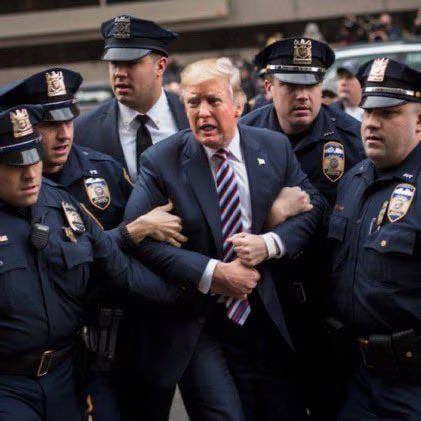
\includegraphics[width=.4\textwidth]{pictures/trump-1.jpg}  \hfill 
   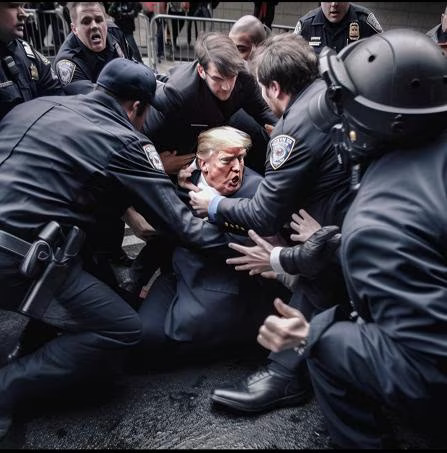
\includegraphics[width=.4\textwidth]{pictures/trump-2.jpg}  


    Queste immagini sono prodotte con il software Midjourney \url{https://www.midjourney.com/}. 
    
    Dopo la registrazione e l'eventuale pagamento dell'abbonamento, si può chiedere la produzione di immagini corrispondenti ad una descrizione a parole.

Le immagini sono realistiche, con pochi difetti formali.  

    \emph{In quale senso i testi di Chat-GPT  e le immagini di Midjourney sono giuste?}

\end{frame}


\end{document}

%%% Local Variables:
%%% reftex-default-bibliography: ("/home/giannidiorestino/Dropbox/InProgress/tutto.bib")
%%% End:

https://www.overleaf.com/project/64109af0a2c0904d6c5e12e8